\documentclass[12pt]{article}
\usepackage{setspace}
\usepackage[procnames]{listings}
\usepackage{color}
\usepackage{graphicx}
\usepackage{cite}
\usepackage{asa}
%\usepackage{endfloat}

% Todo: Remember to update bibtex file
% Todo: Add additional citations...


%\title{Beyond Keywords: Tracking the development of conversations on social media through linked, nested hashtag clusters}
\title{Beyond Keywords: Tracking the evolution of conversational clusters in social media}



\begin{document}
\maketitle

\begin{abstract}
   The potential of social media to give insight into the dynamic evolution of public conversations, and into their reactive and constitutive role in political activities, has to date been underdeveloped. While topic modeling can give static insight into the structure of a conversation, and keyword volume tracking can show how engagement with a specific idea varies over time, there is need for a method of analysis able to understand how conversations about societal values evolve and react to events in the world, incorporating new ideas and relating them to existing themes. In this paper, we propose a method for analyzing social media messages that highlights how world events become connected to existing conversations. This approach has applicability to the study of framing processes, and may reveal how contentious groups connect evolving events to their larger narratives.
\end{abstract}

\doublespacing

\section{Motivation}
	Social media suggests a tantalizing prospect for researchers seeking to understand how newsworthy events influence public and political conversations. Messages on platforms such as Twitter and Facebook represent a high volume sample  of the national conversation in near real time, and with the right handling\footnote{The primary issues involve controlling for demographics. For examples of methods for handling demographic concerns with social media data, see \cite{Bail2015b,McCormick2015}.} can give insight into events such as elections, as demonstrated by \cite{Huberty2013,Tumasjan2010}; or processes such as social movements, as demonstrated by \cite{Agarwal2014,DiGrazia2015}. 
Standard methods of social media analysis use keyword tracking and sentiment analysis to attempt to understand the range of perceptions surrounding these events. 
While helpful for basic situational awareness, these methods do not help us understand how a set of narratives compete to interpret and frame an issue for action.

\begin{figure}[!ht]
  \centering
    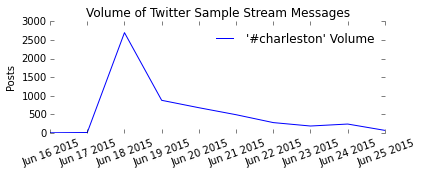
\includegraphics[width=0.85\textwidth]{F1_keyword_volume.png}
    \caption{Standard methods of social media analysis  include keyword volume tracking (shown here),  sentiment analysis, and supervised categorization}
  \label{fig:keyword_vol}
\end{figure}

For example, if we are interested in understanding the national conversation in reaction to the shooting at Emanuel AME church in Charleston, South Carolina in June of 2015, we could plot a timeseries of the volume of tweets containing the hashtag \texttt{\#charleston}, as seen in Figure \ref{fig:keyword_vol}. This tells us something about how many people are engaging with the topic, but little about the ways they are interpreting the event or how they connect the event to their preexisting ideas about gun violence.

Alternate methods include assessing the relative 'positive' or 'negative' sentiment present in these tweets, or using a supervised learning categorizer to group messages according to preconceived ideas about their contents, as demonstrated by \cite{Becker2011,Ritter2010,Zubiaga2011}. Such methods can give aggregated insight into the sentiment expressed, but not into the ways the events are being framed within existing conversations.

Because they look at individual messages and not at the relationships between ideas within messages, these techniques are unable to infer from the data coherent patterns of thought that signify interpretation of the events' deeper meanings. 
Interpretation depends upon making connections between the events as they happen and other concepts in the public discourse. 
One way to measure these connections is to look at a network of co-citations surrounding our topic of interest, as has been demonstrated by \cite{Cogan2012,Smith2014}. 
This technique represents hashtags as nodes on a network, and each message containing two or more hashtags contributes to the weight of an edge between these nodes. 
This type of analysis is helpful in that it helps us begin to understand the structure of the discourse. 
If we perform k-clique clustering on the network, we can see which sets of connections form coherent and conversations, as seen in Figure \ref{fig:basic_clusters}.

\begin{figure}[!ht]
  \centering
    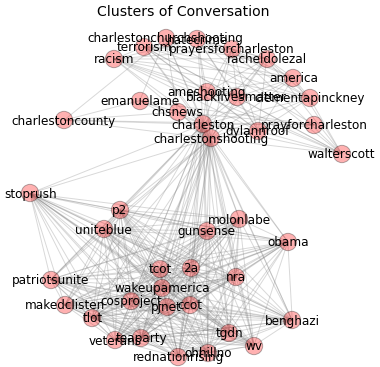
\includegraphics[width=0.65\textwidth]{F2_Basic_Clusters.png}
    \caption{K-clique  clustering  reveals  coherent  structures  in the  hashtag  co-citation  network  that  can  serve  as  proxies  for conversations in the larger national discourse}
  \label{fig:basic_clusters}
\end{figure}

In this example there seem to be two distinct conversations happening with regards to the event: the first a description of the shooting itself and the human elements of the tragedy. 
A second conversation focuses on the larger national-scale political conflicts to which the event points. 
While each of the conversations is motivated by the same event, they are distinct from one another in the language they use and in the connections they draw.

\subsection{The contributions of this paper}
We may hypothesize that how these conversations develop over time will influence the social and political response to the event. 
In this paper we will explore methods of identifying and tracking the development of these conversations over time. We show how these conversation clusters can be identified and visualized, exploring how certain elements form the core of a conversation, while other elements circulate at the periphery. We then demonstrate a method for tracking the evolution of these conversational clusters over time, by relating clusters identified on one day with clusters emerging on subsequent days. This allows us to qualitatively see what new concepts are being included into the discussion, and quantitatively track engagement in these conversations, as distinct from mere references to keywords.

Due to the computation-intensive nature of this analysis, we chose to implement the data manipulation algorithms in both Python and Unicage shell scripts,\footnote{For a description of Unicage development tools, see \cite{Tounaka2013}} for prototyping and speed of execution, respectively. 
Descriptions of these scripts can be found in the appendices, along with performance comparisons between the two languages.

\section{Identifying Conversation Clusters}
The image in Figure \ref{fig:basic_clusters} is based upon network closeness between hashtags. Each of the hashtags present in the dataset forms a node in this network, and the relative strength of edges depends upon the number of times the pair occur together in a tweet, their `co-occurrence', using the method of \cite{Marres}.

The clusters themselves are then defined by k-clique community detection algorithms implemented in the COS Parallel library, developed by \cite{Gregori2013} and their use is demonstrated in the appendices.

\begin{figure}[!ht]
  \centering
    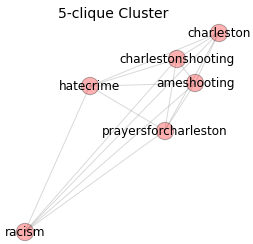
\includegraphics[width=0.45\textwidth]{F3_5clique_clusters.png}
    \caption{Clusters with higher \texttt{k} value are smaller and  more tightly connected, representing a more coherent  or focused conversation}
  \label{fig:5clique}
\end{figure}

Every node in a cluster must be able to participate in at least one fully connected subgroup of size \texttt{k} with the other members of the group. Thus, the metric \texttt{k} determines how strict we are about closeness between keywords when defining the boundaries of a particular cluster. 
For example, high values of \texttt{k} would impose strict requirements for interconnectedness between elements of an identified conversation, leading to a smaller, more coherent identified conversation, as seen in Figure \ref{fig:5clique}.

On the other hand, smaller values of \texttt{k} are less stringent about the requirements of connectivity they put on the elements in the cluster, leading to a larger, more loosely coupled group, as seen in Figure \ref{fig:3clique}.

\begin{figure}[!ht]
  \centering
    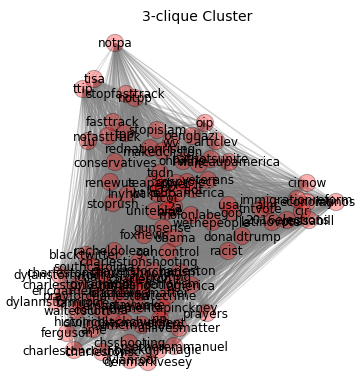
\includegraphics[width=0.65\textwidth]{F4_3clique_clusters.png}
    \caption{Clusters  with  lower  \texttt{k}  value  are  larger  and  less  less  tightly  connected,  representing  more  diffuse  conversation.  They  may  have  smaller  clusters  of  conversation within them}
  \label{fig:3clique}
\end{figure}

\section{Representing Conversational Clusters as Nested Sets}

Tight conversational clusters (high \texttt{k}) must necessarily be contained within larger clusters with less stringent connection requirements (low \texttt{k}). Performing clustering along a range of \texttt{k} values allows us to place a specific conversation in context of the larger discourse. 
It becomes helpful to represent these clusters as nested sets, as seen in Figure \ref{fig:set_cluster}, ignoring the node and edge construction of the network diagram in favor of something which allows us to observe the nested relationships the conversations have with one another.

\begin{figure}[!ht]
  \centering
    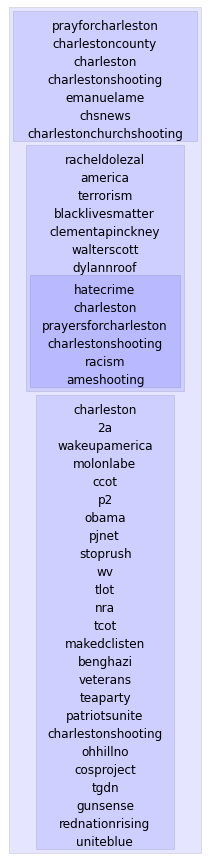
\includegraphics[width=0.3\textwidth]{F5_one_column_nested_cluster.png}
    \caption{Converting networks to nested sets based  upon k-clique clustering simplifies presentation and  analysis of various levels of conversation}
  \label{fig:set_cluster}
\end{figure}
 
In this representation, we are able to observe the tightly clustered 5-clique conversation in context of the 4-clique conversation it inhabits, and the neighboring 4-clique conversations that together inhabit the larger discourse.

\section{Tracking Conversations Chronologically}
In order to track how elements of conversation weave into and out of the general discourse, we need to be able to interpret how conversational clusters identified at one point in time relate to those in subsequent intervals. We can do this in one of two ways. 

The first method is to track the volume of co-citations identified in the various conversational clusters identified on the first day of the analysis, as it changes over subsequent days. This indicates how well the connections made on the first day maintain their relevance in the larger conversation. Figure \ref{fig:cluster_over_time} shows how the connections made in the conversational clusters shown in Figure \ref{fig:set_cluster} fall in volume over the 10 days subsequent to the initial event, paralleling the decay in pure keyword volume seen in Figure \ref{fig:keyword_vol}.

\begin{figure}[!ht]
  \centering
    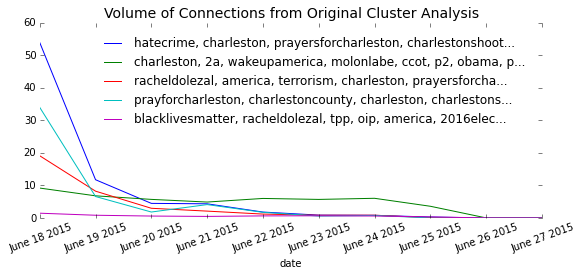
\includegraphics[width=0.9\textwidth]{F6_original_clusters_over_time.png}
    \caption{Tracking the volume of connections made in a single day's clusters (e.g. co-citations) reveals how the specific analogies made immediately after the event maintain their relevance}
  \label{fig:cluster_over_time}
\end{figure}

The second method for tracking conversation volume over time takes into account the changes that happen within the conversation itself. The fundamental assumption in this analysis is that while the words and connections present in a conversation change, they do so incrementally in such a way as to allow for matching conversations during one time period with those in the immediately following time period. 

\cite{Palla2007} discuss how communities of individuals develop over time and change. We can use the same techniques to track continuity of conversational clusters. The most basic way to do this is to count the fraction of elements of a conversational cluster at time 1 that are present in each conversational cluster at time 2, and use this fraction as the likelihood that each cluster at time 2 is an extension or contraction of the time 1 cluster in question. From this we can construct a transition matrix relating conversational clusters at time 1 with clusters at time 2, as seen in Table \ref{tab:transition_matrix}.

\begin{table}[h]
	\caption{A  transition  matrix  contains  the  likelihood  that  a  cluster  at  one  timeperiod  (rows)  corresponds  to  a cluster in the subsequent timeperiod (columns)}
	
	\begin{center}
	  \begin{tabular}{| r | c  c  c  c |}
	    \hline
	    Cluster ID & t2-cl1   & t2-cl2   & t2-cl3   & \ldots \\ \hline
	    t1-cl1     & 0.68     & 0.2      & 0.0      & \ldots \\ 
	    t1-cl2     & 0.0      & 0.85     & 0.03     & \ldots \\
	    t1-cl3     & 0.13     & 0.04     & 0.45     & \ldots \\
	    \ldots     & \ldots   & \ldots   & \ldots   & \ldots \\
	    \hline
	  \end{tabular}
	\end{center}
	\label{tab:transition_matrix}
\end{table}

To improve our estimates, we can take advantage of the fact that clusters that correspond from time 1 to time 2 will participate in a larger cluster that emerges if we perform our clustering algorithm on the union of all edges from the networks at time 1 and time 2. This reduces the number of possible pairings between days, yielding more specificity in our intra-day transition matrices.

\begin{figure}[!ht]
%  \makebox[\textwidth][c]{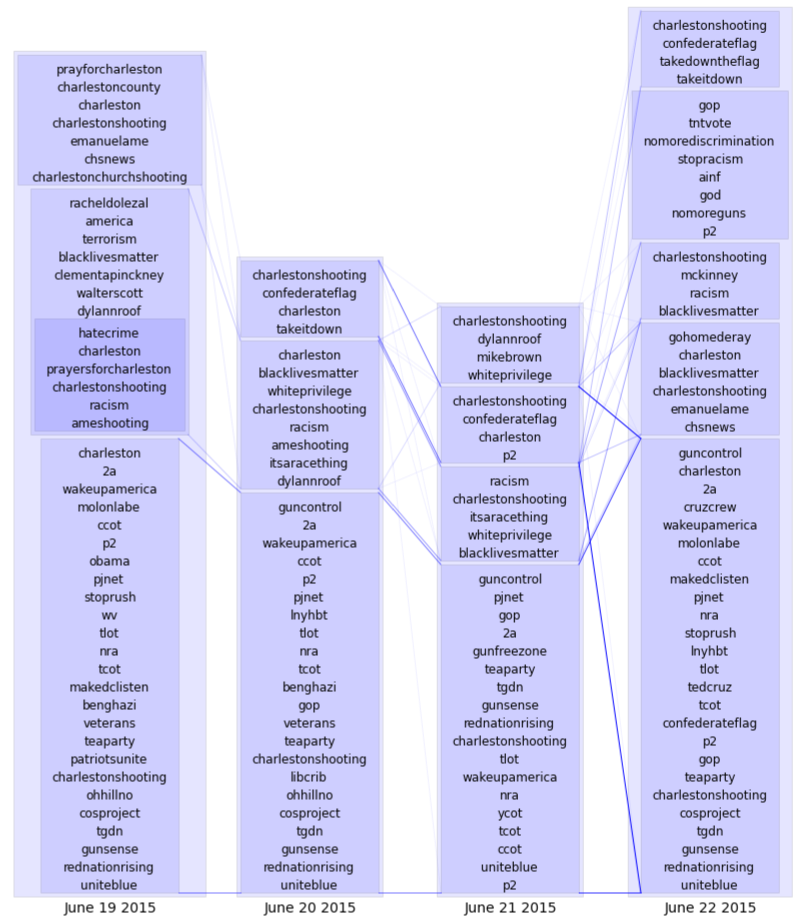
\includegraphics[width=1.1\textwidth]{F7_multi_day_cluster.png}}
  \centering
    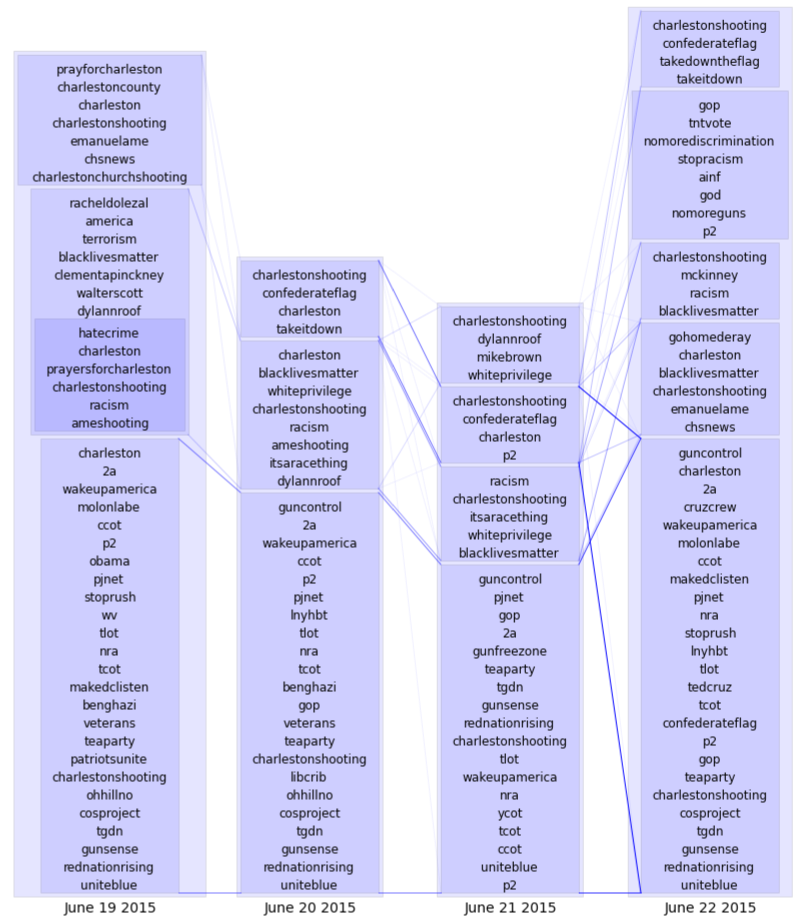
\includegraphics[width=1.0\textwidth]{F7_multi_day_cluster.png}
    \caption{Weighted  traces  connect  conversation  clusters  for  four  days  following  the  shooting. Conversations change over time, as certain components fall out of the cluster, and other components are added}
  \label{fig:multi_day_cluster}
\end{figure}

These transition matrices can be used to infer how clusters present in the first day's analysis correspond to clusters in the second day, and so forth. These are visualized as a set of nested cluster diagrams, with traces linking likely clusters together, as seen in Figure \ref{fig:multi_day_cluster}. Heavier traces between clusters imply more confidence in the transition between the two sets.

\begin{figure}[!ht]
  \centering
    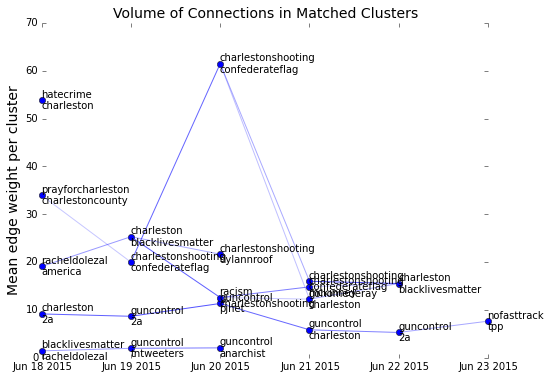
\includegraphics[width=0.9\textwidth]{F8_Matched_cluster_timeseries.png}
    \caption{Plotting over time the mean connection volume in in each conversational cluster,  showing links according to the probabilistic transition matrix. Clusters show relative consistency, with new terms occasionally raising participation}
  \label{fig:cluster_volume_graphs}
\end{figure}

The volume of messages forming the edges of each cluster are shown plotted day by day in Figure \ref{fig:cluster_volume_graphs}. As the linkage between subsequent clusters is probabilistic, in this plot so to are the links connecting volume measures, with the weight of each link proportional to its likelihood. In the present example, we can see how following expressions of the event itself, the conversation evolves into a discussion of the relationship between the violence and the ongoing issue of racism and its connection with the confederate flag. Parallel to and as an undercurrent of these conversations is the ongoing discussion of gun control.

\section{Conclusion}
The utility of social media analysis for sociological research can be extended well beyond the practice of tracking keyword volume, net post sentiment, or supervised classification. In particular, tracking conversational clusters within a network of hashtag co-citations can give both structural understanding of a conversation, and insight into how it develops over time.

These tools can prove helpful to sociologists interested in using social media to understand how world events are framed within the context of existing conversations.

Follow-on work to this paper could attempt to separate the various conversational clusters according to the groups engaged in them, possibly using information about the Twitter connection graph to understand if certain conversations propagate through topologically separate subgraphs, or if multiple conversations occur simultaneously within the same interconnected communities. Such research would have obvious impact on our understanding of framing, polarization, and the formation of group values.

\section{Author's Note}
The appendices to this paper contain all of the code needed to collect necessary data, generate the analysis, and and produce visualizations found herein:

\begin{description}
  \item[Appendix A] Cluster Identification and Transition Analysis in Python
  \item[Appendix B] Cluster Identification and Transition Analysis in Unicage
  \item[Appendix C] Performance Comparison Between Python and Unicage Examples
  \item[Appendix D] Data Collection Scripts
  \item[Appendix E] Visualizations
\end{description}

The full set of scripts, and associated documentation, can be found at \verb|www.github.com\ removed to anonymize|. 


\bibliographystyle{asa}
\bibliography{twitter-clusters}{}

\end{document}
